\documentclass[a4paper,oneside,DIV=10,12pt]{scrartcl}

\usepackage{graphicx}
\usepackage{float}

\usepackage{fontspec}
\setmainfont{STIX Two Text}
\setsansfont{Roboto}

\usepackage{microtype}

\usepackage{polyglossia}
\setmainlanguage{ukrainian}

\usepackage{amsmath}
\usepackage{unicode-math}
\setmathfont{STIX Two Math}
\usepackage[retainorgcmds]{IEEEtrantools}

\usepackage{booktabs}

\usepackage{siunitx}
\sisetup{output-decimal-marker = {,},
exponent-product = {\cdot}}

\usepackage{subcaption}

\begin{document}
	\begin{titlepage}
		\begin{center}
			Міністерство освіти і науки України\\
			Національний авіаційний університет\\
			Навчально-науковий інститут комп'ютерних інформаційних технологій\\
			Кафедра комп'ютеризованих систем управління
			
			\vspace{\fill}
				Лабораторна робота №1\\
				з дисципліни «Теорія електричних та магнітних кіл»\\
				на тему: «Дослідження лінії~передачі електричної~енергії постійним~струмом»\\
				Варіант №
				
			\vspace{\fill}
			
			\begin{flushright}
				Виконав:\\
				студент ННІКІТ СП-225\\
				Клокун Владислав\\
				Перевірив:\\
				Молчанов О.~В.
			\end{flushright}
			Київ 2017
		\end{center}
	\end{titlepage}
	
	\section{Мета роботи}
		\begin{enumerate}
			\item Провести дослідження залежності струму $I$, напруги навантаження $U_{\text{Н}}$, втрати напруги на лінії $U$, потужності генератора $P_{\text{Г}}$, потужності навантаження $P_{\text{Н}}$, втрати потужності на лінії $P$, ККД лінії в залежності від значення опору навантаження при незмінній величині постійної напруги на початку лінії.
			
			\item Дослідити режим, при якому потужність споживача навантаженням досягає свого максимуму.
			
			\item За результатами досліджень виконати необхідні розрахунки, намалювати графічні залежності, зробити висновки.
		\end{enumerate}
		
	\section{Короткі теоретичні відомості}
		Електрична лінія призначена для передачі електричної енергії від генератора до споживача. Найпростіша лінія має два ізольованих проводи, які мають визначений опір. Сумарний опір — $R_{\text{Л}}$.
		
		Струм в лінії при відсутності витоку між проводами дорівнює струму генератора і споживача, тобто по обмотці генератора, лінії і ланцюгам споживача протікає один і той самий струм.
		
		Напруга на навантаженні:
		\[
			U_{\text{Н}} = IR_{\text{Н}} = \frac{U_{\text{Г}}R_{\text{Н}}}{R_{\text{Л}} + R_{\text{Н}}} = \frac{U_{\text{Г}}}{\frac{R_{\text{Л}}}{R_{\text{Н}}} + 1}.
		\]
		
		Втрата напруги $\Delta U$ дорівнює падінню напруги на опорі лінії:
		\[
			\Delta U = U_{\text{Г}} - U_{\text{Н}} = I R_{\text{Л}} = U_{\text{Г}} - \frac{U_{\text{Г}} R_{\text{Н}}}{R_{\text{Л}} + R_{\text{Н}}} = \frac{U^2_{\text{Г}}}{1 + \frac{R_{\text{Н}}}{R_{\text{Л}}}}.
		\]
		
		Потужність генератора:
		\[
			P_{\text{Г}} = U_{\text{Г}} I = \frac{U^2_{\text{Г}}}{R_{\text{Л}} + R_{\text{Н}}}.
		\]
		
		Потужність споживача:
		\[
			P_{\text{Н}} = U_\text{Н} I = \frac{U^2_{\text{Г}} R_{\text{Н}}}{\left( R_{\text{Л}} + R_{\text{Н}} \right)^2} = \frac{U^2_{\text{Г}}}{R_{\text{Н}} + 2R_{\text{Л}}+ \frac{R^2_{\text{Л}}}{R_{\text{Н}}}}.
		\]
		
		Максимальна потужність навантаження:
		\[
			R_{\text{Л}} = R_{\text{Н}}, \quad P_{\text{Н}} = P_{\text{max}} = \frac{U^2_{\text{Г}}}{4 R_{\text{Л}}}
		\]
		
		Максимальна потужність, що передається споживачеві, різко зростає при збільшенні напруги генератора і площі поперечного перерізу проводів.
		
		Втрата потужності на опорі лінії:
		\[
			\Delta P = P_{\text{Г}} - P_{\text{Н}} = I \Delta U = I^2 R_{\text{Л}} = \frac{U^2_{\text{Г}}R_{\text{Л}}}{\left(R_{\text{Л}} + R_{\text{Н}} \right)^2}.
		\]
		
		Коефіцієнт корисної дії:
		\[
			\eta = \frac{P_{\text{Н}}}{P_{\text{Г}}} = \frac{U_{\text{Н}}}{U_{\text{Г}}} = \frac{R_{\text{Н}}}{R_{\text{Л}} + R_{\text{Н}}}.
		\]
		
		При максимальній потужності, що передається споживачеві, ККД дорівнює 50\%. Тому енергетичні лінії використовують у режимах, відмінних від режимів передачі максимальної потужності. Режими передачі максимальної потужності використовують у лініях зв'язку, оскільки ККД для них не є основним показником.
		
	\section{Порядок виконання роботи}
		Зібрати електричну схему (рис. \ref{fig:schematic}). Змінюючи опір навантаження від $0$ до $\infty$ і підтримуючи незмінним задане викладачем значення напруги на вході схеми, зробити необхідні вимірювання за допомогою вимірювальних приладів і занести їх значення у таблицю \ref{tab:measurements}. Кількість дослідів --- 10.
		
		\begin{figure}[!htbp]
			\centering
				\includegraphics[width=0.8\textwidth]{schematic.png}
			\caption{Електрична схема}
			\label{fig:schematic}
		\end{figure}
		
		На основі результатів експерименту розрахувати всі необхідні значення і побудувати графіки залежностей: %$I = f\left(R_{\text{Н}}\right)$, $U_{\text{Н}} = f\left(R_{\text{Н}}\right)$, $\Delta U = f\left(R_{\text{Н}}\right)$, $P_{\text{Г}} = f\left(R_{\text{Н}}\right)$, $P_{\text{Н}} = f\left(R_{\text{Н}}\right)$, $\Delta P = f\left(R_{\text{Н}}\right)$, $\eta = f\left(R_{\text{Н}}\right)$.
		
		\begin{table}[H]
			\centering
			\begin{tabular}{lcr}
			$I = f\left(R_{\text{Н}}\right)$ & $U_{\text{Н}} = f\left(R_{\text{Н}}\right)$ & $\Delta U = f\left(R_{\text{Н}}\right)$\\
			$P_{\text{Г}} = f\left(R_{\text{Н}}\right)$ &  $P_{\text{Н}} = f\left(R_{\text{Н}}\right)$ & $\Delta P = f\left(R_{\text{Н}}\right)$\\
			$\eta = f\left(R_{\text{Н}}\right)$
			\end{tabular}
		\end{table}
		
		Пересвідчитись у тому, що ККД лінії зростає зі збільшенням напруги генератора при одній і тій самій потужності, що виділяється в колі. Для цього треба провести два досліди:
		\begin{enumerate}
			\item Встановити велике значення напруги генератора і порівняно велике значення опору навантаження. Обчислити значення потужності генератора.
			\item Зменшити напругу генератора в два рази, а зміною опору навантаження збільшити струм у колі в два рази.
		\end{enumerate}
		При цьому потужність в обох дослідах однакова. Обчислити значення ККД в цих дослідах і порівняти їх.
		
		% \begin{table}[!htbp]
			% \centering
			% \begin{tabular}{ccccccccc}
			% \toprule
				% \multicolumn{3}{c}{Дослідні дані} & \multicolumn{6}{c}{Розрахункові дані} \\
				% $U_{\text{Г}}, \si{\volt}$ & $U_{\text{Н}}, \si{\volt}$ & $I, \si{\ampere}$ & $\Delta U, \si{\volt}$ & $P_{\text{Г}}, \si{\watt}$ & $P_{\text{Н}}, \si{\watt}$ & $\Delta P, \si{\watt}$ & $\eta, \%$ & $R_{\text{Н}}, \si{\ohm}$\\
			% \midrule
				% \num{10,0} & \num{0} & \num{40e-3} & \num{10} & \num{0,4} & \num{0} & \num{0,4} & 0 & \num{0} \\
				% \num{10,1} & \num{1,6} & \num{34e-3} & \num{8,5} & \num{0,34} & \num{0,054} & \num{0,289} & \num{0,15} & \num{40} \\
				% \num{10,1} & \num{2,7} & \num{30e-3} & \num{7,4} & \num{0,3} & \num{0,081} & \num{0,222} & \num{0,27} & \num{80} \\
				% \num{10,0} & \num{3,5} & \num{27e-3} & \num{6,5} & \num{0,27}  & \num{0,095} & \num{0,1755} & \num{0,35} & \num{120} \\
				% \num{10,0} & \num{4,2} & \num{24e-3} & \num{5,8} & \num{0,24} & \num{0,1} & \num{0,1392} & \num{0,41} & \num{160} \\
				% \num{10,1} & \num{4,9} & \num{21e-3} & \num{5,1} & \num{0,21} & \num{0,102} & \num{0,1071} & \num{0,48} & \num{200} \\
				% \num{10,1} & \num{5,3} & \num{19e-3} & \num{4,8} & \num{0,19} & \num{0,1007} & \num{0,0912} & \num{0,53} & \num{240} \\
				% \num{10,1} & \num{5,7} & \num{17e-3} & \num{4,4} & \num{0,17} & \num{0,09} & \num{0,0748} & \num{0,52} & \num{280} \\
				% \num{10,1} & \num{6,1} & \num{16e-3} & \num{4} &\num{0,16} & \num{0,0976} & \num{0,064} & \num{0,61} & \num{320} \\
				% \num{10,1} & \num{6,4} & \num{15e-3} & \num{3,7} & \num{0,15} & \num{0,096} & \num{0,0555} & \num{0,64} & \num{360} \\
			% \bottomrule
			% \end{tabular}
			% \caption{Вимірювання}
			% \label{tab:measurements}
		% \end{table}
		
		\begin{table}[!htbp]
			\centering
			\begin{tabular}{
				S[table-format=1.1]
				S[table-format=1.1]
				S[table-format=2e2]
				S[table-format=2.1]
				S[table-format=1.2]
				S[table-format=1.4]
				S[table-format=1.4]
				S[table-format=2]
				S[table-format=3.0]%, table-number-alignment=right]
			}
			\toprule
				\multicolumn{3}{c}{Дослідні дані} & \multicolumn{6}{c}{Розрахункові дані} \\
				\cmidrule(lr){1-3} \cmidrule(lr){4-9}
				{$U_{\text{Г}}, \si{\volt}$} & {$U_{\text{Н}}, \si{\volt}$} & {$I, \si{\ampere}$} & {$\Delta U, \si{\volt}$} & {$P_{\text{Г}}, \si{\watt}$} & {$P_{\text{Н}}, \si{\watt}$} & {$\Delta P, \si{\watt}$} & {$\eta, \%$} & {$R_{\text{Н}}, \si{\ohm}$}\\
				
			\midrule
				10,0 & 0 & 40e-3 & 10 & 0,4 & 0 & 0,4 & 0 & 0 \\
				10,1 & 1,6 & 34e-3 & 8,5 & 0,34 & 0,054 & 0,289 & 15 & 40 \\
				10,1 & 2,7 & 30e-3 & 7,4 & 0,3 & 0,081 & 0,222 & 27 & 80 \\
				10,0 & 3,5 & 27e-3 & 6,5 & 0,27  & 0,095 & 0,1755 & 35 & 120 \\
				10,0 & 4,2 & 24e-3 & 5,8 & 0,24 & 0,1 & 0,1392 & 41 & 160 \\
				10,1 & 4,9 & 21e-3 & 5,1 & 0,21 & 0,102 & 0,1071 & 48 & 200 \\
				10,1 & 5,3 & 19e-3 & 4,8 & 0,19 & 0,1007 & 0,0912 & 53 & 240 \\
				10,1 & 5,7 & 17e-3 & 4,4 & 0,17 & 0,09 & 0,0748 & 52 & 280 \\
				10,1 & 6,1 & 16e-3 & 4 &0,16 & 0,0976 & 0,064 & 61 & 320 \\
				10,1 & 6,4 & 15e-3 & 3,7 & 0,15 & 0,096 & 0,0555 & 64 & 360 \\
			\bottomrule
			\end{tabular}
			\caption{Вимірювання}
			\label{tab:measurements}
		\end{table}
		
		За отриманими дослідними і розрахунковими даними (табл.~\ref{tab:measurements}) будуємо графіки шуканих залежностей (рис.~\ref{fig:plots}).
		
		\begin{figure}
		\centering
			\begin{subfigure}[b]{0.49\textwidth}
				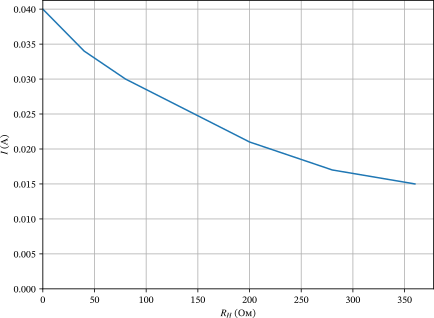
\includegraphics[width=\textwidth]{01-i-edited.pdf}
				\caption{$I = f(R_{\text{Н}})$}
			\end{subfigure}
			~
			\begin{subfigure}[b]{0.49\textwidth}
				\includegraphics[width=\textwidth]{02-u-nag-edited.pdf}
				\caption{$U_{\text{Н}} = f(R_{\text{Н}})$}
			\end{subfigure}
			
			\vspace*{\floatsep}
			
			\begin{subfigure}[b]{0.49\textwidth}
				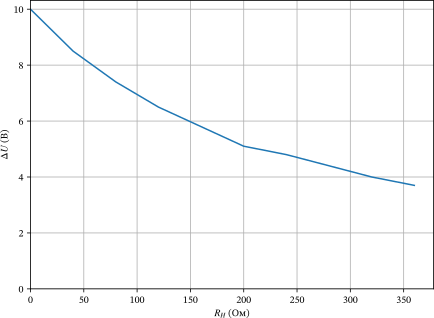
\includegraphics[width=\textwidth]{03-delta-u-edited.pdf}
				\caption{$\Delta U = f(R_{\text{Н}})$}
			\end{subfigure}
			~
			\begin{subfigure}[b]{0.49\textwidth}
				\includegraphics[width=\textwidth]{04-p-gen-edited.pdf}
				\caption{$P_{\text{Г}} = f(R_{\text{Н}})$}
			\end{subfigure}
			
			\vspace*{\floatsep}
			
			\begin{subfigure}[b]{0.49\textwidth}
				\includegraphics[width=\textwidth]{05-p-nag-edited.pdf}
				\caption{$P_{\text{Н}} = f(R_{\text{Н}})$}
			\end{subfigure}
			~
			\begin{subfigure}[b]{0.49\textwidth}
				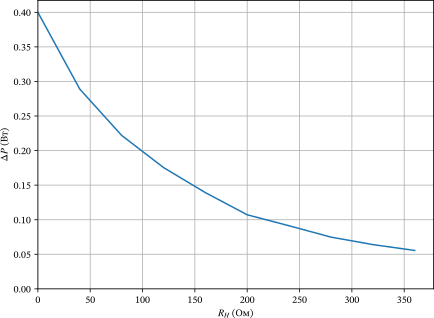
\includegraphics[width=\textwidth]{06-delta-p-edited.pdf}
				\caption{$\Delta P = f(R_{\text{Н}})$}
			\end{subfigure}
		\caption{Графіки залежностей різних величин від $R_{\text{Н}}$}
		\end{figure}
		
		\begin{figure}
		\centering
		\ContinuedFloat
			\begin{subfigure}{\textwidth}
				\includegraphics[width=\textwidth]{07-eta-edited.pdf}
				\caption{$\eta = f(R_{\text{Н}})$}
			\end{subfigure}
		\caption{Графіки залежностей різних величин від $R_{\text{Н}}$}
		\label{fig:plots}
		\end{figure}
		
	\section{Висновки}
		Виконуючи дану лабораторну роботу, ми провели дослідження залежності струму $I$, напруги навантаження $U_{\text{Н}}$, втрати напруги на лінії $U$, потужності генератора $P_{\text{Г}}$, потужності навантаження $P_{\text{Н}}$, втрати потужності на лінії $P$, ККД лінії в залежності від значення опору навантаження при незмінній величині постійної напруги на початку лінії. Дослідили режим, при якому потужність споживача навантаженням досягає свого максимуму. За результатами досліджень виконали необхідні розрахунки та намалювали графічні залежності.
\end{document}
